\documentclass{wileysev}

\usepackage[T1]{fontenc}
\usepackage[utf8]{inputenc}
\usepackage{amsmath,amssymb,amsfonts,mathtools}
\usepackage{bm}
\usepackage{graphicx}
\graphicspath{{figs/}}
\usepackage{booktabs}
\usepackage{array}
\usepackage{float}
\usepackage{multirow}
\usepackage{tikz}
\usepackage{pgfplots}
\usetikzlibrary{arrows.meta,positioning,calc,decorations.pathreplacing}
\pgfplotsset{compat=1.18}
\usepackage{mdframed}
\usepackage{xcolor}

% Color palette
\definecolor{cBlue}{RGB}{55,138,221}
\definecolor{cRed}{RGB}{226,75,74}
\definecolor{cPurple}{RGB}{127,119,221}
\definecolor{cGreen}{RGB}{58,130,60}
\definecolor{cAmber}{RGB}{186,117,23}
\definecolor{cPanel}{RGB}{250,249,247}
\definecolor{cBorder}{RGB}{205,203,196}
\definecolor{cText}{RGB}{38,38,36}
\definecolor{cMuted}{RGB}{130,128,122}
\definecolor{cGoodBg}{RGB}{234,243,222}
\definecolor{cBadBg}{RGB}{252,235,235}
\definecolor{cPurpleBg}{RGB}{238,237,254}
\definecolor{cInfoBg}{RGB}{230,241,251}
\definecolor{cAmberBg}{RGB}{250,238,218}
\definecolor{cStrip}{RGB}{238,236,230}

% TikZ styles
\tikzset{
	panbox/.style={draw=cBorder,line width=0.5pt,rounded corners=4pt,fill=cPanel},
	arr/.style={-{Stealth[length=3.5pt,width=2.8pt]},line width=0.9pt},
	goodbox/.style={draw=cGreen!60,line width=0.5pt,rounded corners=3pt,
		fill=cGoodBg,inner sep=4pt,align=center},
	badbox/.style={draw=cRed!60,line width=0.5pt,rounded corners=3pt,
		fill=cBadBg,inner sep=4pt,align=center},
	infobox/.style={draw=cBlue!40,line width=0.5pt,rounded corners=3pt,
		fill=cInfoBg,inner sep=4pt,align=center},
	amberbox/.style={draw=cAmber!60,line width=0.5pt,rounded corners=3pt,
		fill=cAmberBg,inner sep=4pt,align=center},
	ax/.style={-{Stealth[length=3pt,width=2.4pt]},line width=0.5pt,color=cMuted},
}



% Minimal black/white figure styles used by the combined rigorous version.
% The older colored styles are kept for compatibility with tables/callouts, but
% the main explanatory diagrams below use these sparse styles.
\tikzset{
	mbox/.style={draw=black!75, line width=0.45pt, rounded corners=2pt,
		fill=white, inner xsep=6pt, inner ysep=5pt, align=center,
		font=\scriptsize},
	msmall/.style={draw=black!75, line width=0.45pt, rounded corners=1.5pt,
		fill=white, inner xsep=4pt, inner ysep=3pt, align=center,
		font=\scriptsize},
	simbox/.style={draw=black!75, line width=0.45pt, rounded corners=2pt,
		fill=white, inner xsep=7pt, inner ysep=6pt, align=center,
		font=\small},
	marr/.style={-{Stealth[length=3pt,width=2.3pt]}, line width=0.55pt,
		draw=black!70},
	mloop/.style={-{Stealth[length=3pt,width=2.3pt]}, line width=0.55pt,
		draw=black!60, dashed},
	maxis/.style={-{Stealth[length=2.7pt,width=2pt]}, line width=0.45pt,
		draw=black!55},
}

% Custom callout environments
\newmdenv[backgroundcolor=cInfoBg,linecolor=cBlue!50,linewidth=0.6pt,
roundcorner=4pt,skipabove=6pt,skipbelow=6pt,
innerleftmargin=8pt,innerrightmargin=8pt,
innertopmargin=5pt,innerbottommargin=5pt]{infoenv}
\newmdenv[backgroundcolor=cGoodBg,linecolor=cGreen!60,linewidth=0.6pt,
roundcorner=4pt,skipabove=6pt,skipbelow=6pt,
innerleftmargin=8pt,innerrightmargin=8pt,
innertopmargin=5pt,innerbottommargin=5pt]{goodenv}
\newmdenv[backgroundcolor=cAmberBg,linecolor=cAmber!60,linewidth=0.6pt,
roundcorner=4pt,skipabove=6pt,skipbelow=6pt,
innerleftmargin=8pt,innerrightmargin=8pt,
innertopmargin=5pt,innerbottommargin=5pt]{amberenv}
\newmdenv[backgroundcolor=cBadBg,linecolor=cRed!50,linewidth=0.6pt,
roundcorner=4pt,skipabove=6pt,skipbelow=6pt,
innerleftmargin=8pt,innerrightmargin=8pt,
innertopmargin=5pt,innerbottommargin=5pt]{warnenv}

% Old class + hyperref safety
\setlength{\paperwidth}{8.5in}
\setlength{\paperheight}{11in}

\usepackage{hyperref}
\usepackage[nameinlink,noabbrev]{cleveref}

% Suppress the class's forced odd-page section starts.
\makeatletter
\@openrightfalse
\let\cleardoublepage\clearpage
\def\startonoddpage{\clearpage}
\makeatother

% -------------------------------------------------
% Title-page metadata
% -------------------------------------------------
\booktitle{JUNA: A Joint Receiver for Doppler-Resilient OFDM}
\subtitle{Partial-FFT Coefficient Estimation and LDPC-Coupled Detection}
\authors{
	Gabriel Chua
	\affil{ARL, National University of Singapore}
	\affil{\today}
}
\offprintinfo{Project SONIQUE -- D1 draft 1.1}{Gabriel Chua}
\editionstatement{ARL Project Report}

% -------------------------------------------------
% Handy macros
% -------------------------------------------------
\newcommand{\C}{\mathbb{C}}
\newcommand{\R}{\mathbb{R}}
\newcommand{\F}{\mathbb{F}}
\newcommand{\E}{\mathbb{E}}
\newcommand{\Ht}{^{H}}
\newcommand{\T}{^{T}}
\newcommand{\norm}[1]{\left\lVert #1 \right\rVert}
\newcommand{\abs}[1]{\left\lvert #1 \right\rvert}

\begin{document}
	
	\frontmatter
	\halftitlepage
	\titlepage
	\tableofcontents
	
	\acronyms
	\acro{OFDM}{Orthogonal frequency-division multiplexing}
	\acro{CP}{Cyclic prefix}
	\acro{ICI}{Inter-carrier interference}
	\acro{LDPC}{Low-density parity-check}
	\acro{LLR}{Log-likelihood ratio}
	\acro{FFT}{Fast Fourier transform}
	\acro{LS}{Least squares}
	\acro{RLS}{Recursive least squares}
	\acro{RPC}{RLS-based Partial-FFT Combiner}
	\acro{DFEC}{Differentiable forward error correction}
	\acro{BP}{Belief propagation}
	\acro{QPSK}{Quadrature phase-shift keying}
	\acro{AWGN}{Additive white Gaussian noise}
	\acro{SNR}{Signal-to-noise ratio}
	\acro{SFM}{Spectral flatness measure}
	\acro{STD}{Standard one-tap receiver}
	\acro{SPA}{Sum-product algorithm}
	\acro{LMMSE}{Linear minimum mean-square error}
	\acro{AD}{Automatic differentiation}
	\acro{BER}{Bit error rate}
	\acro{EVM}{Error vector magnitude}
	\acro{CSI}{Channel state information}
	\acro{JUNA}{Joint Unified Nonideality-Aware Algorithm}
	\endacronyms
	
	\clearpage
	\begin{table}[H]
		\caption{Notation used in the remainder of the paper.}
		\label{tab:notation}
		\centering
		\scriptsize
		\setlength{\tabcolsep}{4pt}
		\renewcommand{\arraystretch}{1.0}
		
		\begin{minipage}[t]{0.49\textwidth}
			\vspace{0pt}
			\centering
			\begin{tabular}{@{} l p{0.68\linewidth} @{}}
				\toprule
				\multicolumn{2}{@{}l}{\textbf{OFDM and Channel Model}}\\
				\midrule
				$N$ & number of OFDM subcarriers\\
				$N_{\mathrm{cp}}$ & cyclic prefix length\\
				$\mathcal{K}$ & active-carrier index set\\
				$\mathcal{P}$ & pilot-carrier index set\\
				$\mathcal{D}$ & data-carrier index set\\
				$X_k$ & transmitted symbol on carrier $k$\\
				$Y_k$ & received symbol on carrier $k$\\
				$\widehat H_k$ & pilot-estimated channel frequency response\\
				$L_h$ & time-domain channel-estimation length\\
				$\rho_{\mathrm{LS}}$ & ridge weight in pilot-LS channel estimation\\
				$H_{k\ell}(a)$ & fixed-Doppler frequency-domain coupling from carrier $\ell$ to $k$\\
				$\nu_k$ & frequency-domain additive noise on carrier $k$\\
				$\bm{\nu}_{\mathrm{t}}$ & time-domain additive noise vector\\
				$\bm{\nu}$ & frequency-domain additive noise vector\\
				
				\midrule
				\multicolumn{2}{@{}l}{\textbf{Partial-FFT Reception}}\\
				\midrule
				$M$ & number of partial-FFT branches\\
				$Y_{k,m}$ & partial-FFT observation on carrier $k$, branch $m$\\
				$\mathbf{Y}_k$ & partial-FFT observation vector for carrier $k$\\
				$\mathbf{W}_k$ & combining vector for carrier $k$\\
				$\widetilde{X}_k$ or $\widehat{s}_k$ & pre-decoder scalar soft symbol on carrier $k$\\
				$\mathbf{C}$ & branch-domain local ICI/nonideality parameters\\
				$\mathbf{c}_{k,q}$ & branch response from carrier $q$ to carrier $k$\\
				$\Sigma_k$ & branch-noise covariance for carrier $k$\\
				\bottomrule
			\end{tabular}
		\end{minipage}\hfill
		\begin{minipage}[t]{0.49\textwidth}
			\vspace{0pt}
			\centering
			\begin{tabular}{@{} l p{0.68\linewidth} @{}}
				\toprule
				\multicolumn{2}{@{}l}{\textbf{RPC Combiner}}\\
				\midrule
				$\mathcal{P}(k)$ & nearby pilot set used for carrier $k$\\
				$\delta$ & ridge parameter in the RPC fit\\
				$\mathbf{U}_k$ & stacked pilot observation matrix for carrier $k$\\
				$\mathbf{d}_k$ & stacked pilot symbol vector for carrier $k$\\
				$\mathbf{R}_k$ & pilot correlation matrix\\
				$\mathbf{r}_k$ & pilot cross-correlation vector\\
				$\beta$ & forgetting factor in the RLS recursion\\
				$\widehat X_k$ & one-tap equalized symbol using $\widehat H_k$\\
				
				\midrule
				\multicolumn{2}{@{}l}{\textbf{Channel Metrics}}\\
				\midrule
				$\mathrm{SFM}$ & spectral flatness measure\\
				$D_{\mathrm{notch}}$ & max-to-min frequency-response notch depth\\
				$\bar{\eta}$ & mean ICI ratio from $H_{k\ell}(a)$\\
				
				\midrule
				\multicolumn{2}{@{}l}{\textbf{JUNA and LDPC}}\\
				\midrule
				$\mathbf{W}$ & collection of all per-carrier combining vectors\\
				$\mathbf{z}$ & bit-level latent optimization variables\\
				$\xi_i(\mathbf{z})$ & relaxed bipolar coded bit, $\tanh z_i$\\
				$s_k(\mathbf{z})$ & relaxed QPSK symbol induced by two coded bits\\
				$K_{\mathrm{ICI}}$ & half-bandwidth of the local ICI model\\
				$\mathbf{P}$ & LDPC parity-check matrix\\
				$\{\mathcal{N}_j\}$ & parity-check neighborhoods\\
				$\mathcal B_K(k)$ & local ICI neighborhood around carrier $k$\\
				$\mathcal{A}_k(\mathbf{C},\mathbf{s})$ & branch-domain forward model on carrier $k$\\
				$\lambda_{\mathrm{d}}$ & weight of the signal term\\
				$\eta$ & weight of the pilot term\\
				$\gamma_C,\gamma_W,\gamma_S$ & weights for branch model, combiner energy, and combiner smoothness\\
				$\rho$ & weight tying scalar combiner outputs to relaxed data symbols\\
				$\lambda_{\mathrm{p}}$ & weight of the soft parity-check penalty\\
				\bottomrule
			\end{tabular}
		\end{minipage}
	\end{table}
	\clearpage
	
	\mainmatter
	
	\section{Introduction}
	\label{chap:introduction}
	
	Orthogonal frequency-division multiplexing (OFDM) relies on the channel being slow enough that the frequency-domain input--output relation is approximately diagonal. Under residual Doppler this assumption breaks down: even after packet acquisition and coarse Doppler correction, the channel varies within the OFDM interval, subcarrier orthogonality is destroyed, inter-carrier interference (ICI) emerges, and pilot-only equalization fails. The receiver must then estimate reliable \emph{pre-decoder soft symbols} --- the soft subcarrier estimates supplied to the LDPC decoder --- under structured intra-symbol time variation.
	
	This report develops the receiver argument in four steps. First, we establish the CP-OFDM baseline without Doppler or platform motion, then show how residual Doppler converts the diagonal operator into a banded one (Section~\ref{chap:doppler}). Second, we survey conventional defenses against this breakdown --- comb pilots, partial-FFT temporal slicing, and the RLS-based Partial-FFT Combiner (RPC) --- and identify the point at which separating RPC from LDPC decoding starts to hurt (Section~\ref{chap:defenses}). Third, we introduce \emph{JUNA} (Joint Unified Nonideality-Aware Algorithm), a coupled formulation in which soft-symbol estimation and LDPC-constrained decoding share a single objective so that pilots, channel structure, and code constraints regularize one another throughout inference (Section~\ref{chap:juna}). The remaining sections present an alternating solver (Section~\ref{chap:solver}) and a packet-level validation across a population of underwater acoustic channels (Section~\ref{chap:results}).
	
	The joint approach adapts principles from differentiable forward error correction (DFEC) from ISI channels to Doppler-distorted OFDM, and is most useful where local pilot information alone is insufficient: sparse pilots, strong residual Doppler, and mid-to-low SNR where decision-directed updates become unreliable.
	
	\section{The Diagonal OFDM Model and Residual Doppler}
	\label{chap:doppler}
	
	\subsection{Pristine CP-OFDM and the Diagonal Model}
	\label{ssec:diagonal_baseline}
	
	Consider an OFDM system with \(N\) subcarriers and cyclic prefix of length \(N_{\mathrm{cp}}\), pilot set \(\mathcal{P}\) and data set \(\mathcal{D}\). Let \(\mathbf{X}=[X_0,\dots,X_{N-1}]^{T}\in\C^N\) denote one frequency-domain OFDM symbol and \(\mathbf{F}\) the unitary \(N\times N\) DFT matrix. The useful time-domain block is \(\mathbf{x}=\mathbf{F}^{H}\mathbf{X}\). After CP insertion, transmission through an \(L\)-tap channel with \(L-1\le N_{\mathrm{cp}}\), and CP removal, the received block satisfies
	\begin{equation}
		\mathbf{r} = \mathbf{H}_{\mathrm{cir}}\mathbf{x} + \bm{\nu}_{\mathrm{t}},
		\label{eq:circulant_block_model}
	\end{equation}
	with \(\mathbf{H}_{\mathrm{cir}}\) circulant. Applying the FFT then gives
	\begin{equation}
		\mathbf{Y}
		=
		\mathbf{F}\mathbf{r}
		=
		\mathbf{F}\mathbf{H}_{\mathrm{cir}}\mathbf{F}^{H}\mathbf{X}
		+
		\mathbf{F}\bm{\nu}_{\mathrm{t}}
		=
		\operatorname{diag}(\mathbf{H})\mathbf{X}
		+
		\bm{\nu},
		\label{eq:nominal_diagonal_ofdm}
	\end{equation}
	the familiar one-tap OFDM model: each active subcarrier satisfies \(Y_k = H_k X_k + \nu_k\), and post-equalization reliability depends only on accurate estimation of the per-carrier channel gains \(H_k\). This diagonal baseline is the pristine state of the channel operator. Everything that follows is a perturbation of it.
	
	\subsection{Packet Time-Scaling Under Doppler}
	\label{ssec:time_scaling}
	
	Doppler distortion acts as a time-scaling of the received waveform: if the transmitted packet is \(s(t)\), the received signal is
	\begin{equation}
		r(t) = s\!\big((1+a)t\big),
		\label{eq:time_scaling_intro}
	\end{equation}
	where \(a\) is the Doppler scale. The packet is compressed for \(a>0\) and stretched for \(a<0\), so sample locations shift from the nominal OFDM symbol grid. Coarse Doppler correction reduces the global mismatch but leaves residual intra-symbol variation, which breaks the circulant structure of~\eqref{eq:circulant_block_model}: the received OFDM symbol no longer aligns with the nominal FFT basis window.
	
	\subsection{Loss of Subcarrier Orthogonality}
	\label{ssec:orthogonality_loss}
	
	The diagonal model~\eqref{eq:nominal_diagonal_ofdm} required orthogonal subcarriers over the useful interval. Residual Doppler destroys that orthogonality: the waveform no longer matches the nominal basis, and energy leaks between subcarriers. The frequency-domain model becomes
	\begin{equation}
		Y_k = H_{k,k}X_k + \sum_{\ell \neq k} H_{k,\ell}X_\ell + \nu_k,
		\label{eq:doppler_freq_coupling_intro}
	\end{equation}
	where the off-diagonal terms \(H_{k,\ell}\) represent Doppler-induced ICI. The receiver must now estimate both the transmitted symbols and how Doppler couples the observations. Figure~\ref{fig:doppler_offdiag_concept} illustrates the transition: the nominal channel is diagonal; residual Doppler causes basis mismatch within the FFT window, off-diagonal leakage in the frequency-domain operator, and visible phase smearing in the received constellation. One-tap pilot-only equalization, which assumes~\eqref{eq:nominal_diagonal_ofdm}, becomes unreliable in this regime.
	
	
	\begin{figure}[tbp]
		\centering
		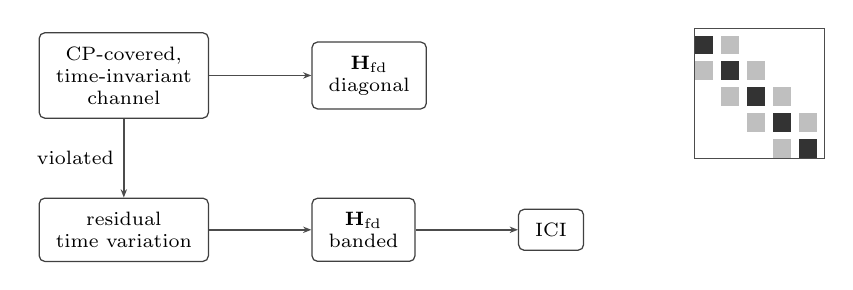
\begin{tikzpicture}[node distance=13mm]
			\node[mbox] (ideal) {CP-covered,\\time-invariant\\channel};
			\node[mbox, right=of ideal] (diag) {$\mathbf H_{\rm fd}$\\diagonal};
			\node[mbox, below=10mm of ideal] (dop) {residual\\time variation};
			\node[mbox, right=of dop] (band) {$\mathbf H_{\rm fd}$\\banded};
			\node[mbox, right=of band] (ici) {ICI};
			\draw[marr] (ideal) -- (diag);
			\draw[marr] (dop) -- (band);
			\draw[marr] (band) -- (ici);
			\draw[marr] (ideal) -- node[left,font=\scriptsize] {violated} (dop);
			\begin{scope}[shift={(7.25,-1.05)}, scale=0.33]
				\draw[black!70] (0,0) rectangle (5,5);
				\foreach \i in {0,...,4}{
					\foreach \j in {0,...,4}{
						\pgfmathtruncatemacro{\dist}{abs(\i-\j)}
						\ifnum\dist=0
						\fill[black!80] (\j,4-\i) rectangle +(0.72,0.72);
						\else\ifnum\dist=1
						\fill[black!25] (\j,4-\i) rectangle +(0.72,0.72);
						\fi\fi
					}
				}
			\end{scope}
		\end{tikzpicture}
		\caption{Minimal residual-Doppler picture. A CP-covered time-invariant channel is diagonal in the OFDM basis. Residual time variation makes the frequency-domain operator non-diagonal; under local Doppler the dominant off-diagonal terms are near the main diagonal.}
		\label{fig:doppler_offdiag_concept}
	\end{figure}
	
	
	\subsection{Residual Time Variation and Banded Structure}
	\label{ssec:banded_structure}
	
	The scalar coupling model~\eqref{eq:doppler_freq_coupling_intro} can be written more precisely as an operator perturbation. Let \(\mathbf G\) denote the post-acquisition, CP-removed time-domain channel operator over one useful OFDM block. In the ideal CP-covered time-invariant case, \(\mathbf G=\mathbf H_{\mathrm{cir}}\) is circulant and the diagonal model~\eqref{eq:nominal_diagonal_ofdm} follows. Under residual time variation,
	\begin{equation}
		\mathbf r
		= \mathbf G\mathbf F^{H}\mathbf X + \bm\nu_{\mathrm t},
		\qquad
		\mathbf Y
		= \mathbf F\mathbf G\mathbf F^{H}\mathbf X+\bm\nu
		\triangleq \mathbf H_{\mathrm{fd}}\mathbf X+\bm\nu .
		\label{eq:fd_matrix_model}
	\end{equation}
	Thus the diagonal OFDM model is not an assumption about OFDM alone; it follows from the joint assumptions of CP-covered delay spread, correct timing, and channel invariance over the useful interval. Residual Doppler violates the last condition, so \(\mathbf G\) is generally non-circulant and \(\mathbf H_{\mathrm{fd}}\) is generally non-diagonal.
	
	For local Doppler distortions, the off-diagonal energy of \(\mathbf H_{\mathrm{fd}}\) is usually concentrated near the main diagonal. We therefore use the banded approximation
	\begin{equation}
		Y_k
		= H_{k,k}X_k
		+ \sum_{q\in\mathcal B_K(k)\setminus\{k\}} H_{k,q}X_q
		+ \nu_k,
		\qquad
		\mathcal B_K(k)=\{q\in\mathcal K: |q-k|\le K_{\mathrm{ICI}}\}.
		\label{eq:rigorous_banded_ici}
	\end{equation}
	The truncation error is
	\begin{equation}
		\epsilon_k^{(K)}
		= \sum_{q\notin\mathcal B_K(k)}H_{k,q}X_q,
		\qquad
		\mathbb E|\epsilon_k^{(K)}|^2
		= \sum_{q\notin\mathcal B_K(k)} |H_{k,q}|^2\mathbb E|X_q|^2,
		\label{eq:rigorous_truncation_error}
	\end{equation}
	for independent zero-mean symbols. Increasing \(K_{\mathrm{ICI}}\) reduces model bias but increases the number of front-end coefficients to estimate. Figure~\ref{fig:doppler_offdiag_concept} summarizes this operator-level transition, and Figure~\ref{fig:typical_ofdm_chain} situates the receiver blocks affected by the loss of diagonality.
	
	
	\begin{figure}[tbp]
		\centering
		\resizebox{\textwidth}{!}{%
		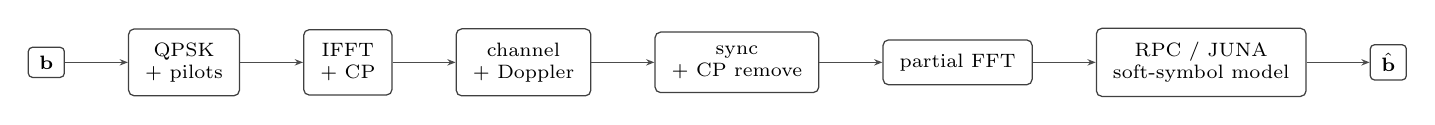
\begin{tikzpicture}[node distance=8mm]
			\node[msmall] (bits) {$\mathbf b$};
			\node[mbox, right=of bits] (map) {QPSK\\+ pilots};
			\node[mbox, right=of map] (ifft) {IFFT\\+ CP};
			\node[mbox, right=of ifft] (chan) {channel\\+ Doppler};
			\node[mbox, right=of chan] (sync) {sync\\+ CP remove};
			\node[mbox, right=of sync] (pfft) {partial FFT};
			\node[mbox, right=of pfft] (juna) {RPC / JUNA\\soft-symbol model};
			\node[msmall, right=of juna] (out) {$\hat{\mathbf b}$};
			\draw[marr] (bits) -- (map);
			\draw[marr] (map) -- (ifft);
			\draw[marr] (ifft) -- (chan);
			\draw[marr] (chan) -- (sync);
			\draw[marr] (sync) -- (pfft);
			\draw[marr] (pfft) -- (juna);
			\draw[marr] (juna) -- (out);
		\end{tikzpicture}}
		\caption{Minimal packet-processing chain. The receiver-specific contribution begins after synchronization and CP removal, where partial-FFT observations are passed to the soft-symbol estimator and LDPC-coupled detector.}
		\label{fig:typical_ofdm_chain}
	\end{figure}
	
	\section{Conventional Defenses Against ICI}
	\label{chap:defenses}
	
	Residual Doppler leaves a banded operator~\eqref{eq:fd_matrix_model} in place of the diagonal baseline~\eqref{eq:nominal_diagonal_ofdm}. This section surveys three layers of conventional response to that breakdown --- comb pilots for channel anchoring, partial-FFT reception for richer observations, and the RLS-based Partial-FFT Combiner (RPC) for pilot-trained soft-symbol formation --- and identifies the point at which separate RPC and decoding begin to hurt under sparse pilots and strong Doppler. That limit is what JUNA is designed to address.
	
	\subsection{Pilot Anchors and Comb Placement}
	\label{ssec:pilot-grid}
	
	Active subcarriers are assigned as pilot, data, or null. A \emph{comb pilot pattern} places pilots at regular intervals (every \(S\)-th subcarrier), giving \(N_{\mathrm{pil}}=N_{\mathrm{act}}/S\) pilot tones. Density trades estimation accuracy against payload capacity: denser pilots track Doppler better but cost throughput. The comb placement, illustrated in Figure~\ref{fig:pilot-grid}, is used throughout the remainder of the report.
	
	On a pilot tone \(k\in\mathcal{P}\) with known symbol \(P_k\), the pilot least-squares estimate of the local diagonal gain is \(\hat H_k^{\mathrm{LS}} = Y_k/P_k\), unbiased with variance \(\sigma^2/|P_k|^2\). Data-tone estimates are obtained by interpolation from nearby pilots. This interpolation-based picture assumes a diagonal operator and therefore breaks under the off-diagonal leakage of~\eqref{eq:doppler_freq_coupling_intro}: one tap per carrier is simply not enough degrees of freedom to represent a banded response. The natural next step is to give the receiver more observations per carrier.
	
	
	\begin{figure}[tbp]
		\centering
		\resizebox{0.95\textwidth}{!}{%
		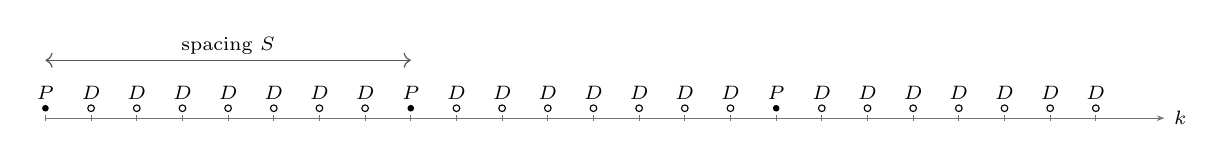
\begin{tikzpicture}[x=0.58cm,y=0.7cm]
			\draw[maxis] (0,0) -- (24.5,0) node[right,font=\scriptsize] {$k$};
			\foreach \k in {0,...,23}{
				\pgfmathtruncatemacro{\m}{mod(\k,8)}
				\draw[black!55] (\k,0.05) -- (\k,-0.05);
				\ifnum\m=0
				\node[font=\scriptsize] at (\k,0.45) {$P$};
				\fill[black] (\k,0.18) circle (1.2pt);
				\else
				\node[font=\scriptsize] at (\k,0.45) {$D$};
				\fill[white,draw=black] (\k,0.18) circle (1.2pt);
				\fi
			}
			\draw[<->,line width=0.45pt,draw=black!65] (0,1.05) -- (8,1.05);
			\node[font=\scriptsize] at (4,1.32) {spacing $S$};
		\end{tikzpicture}}
		\caption{Comb pilot pattern. Known pilots are inserted every $S$ active carriers; intervening carriers carry coded QPSK data.}
		\label{fig:pilot-grid}
	\end{figure}
	
	
	\subsection{Temporal Slicing: Partial-FFT Reception}
	\label{ssec:partial-fft}
	
	A conventional receiver represents each active carrier by a single FFT output. Partial-FFT reception instead decomposes the useful OFDM interval into \(M\) temporal components and computes one FFT contribution per component. Let \(g_m[n]\), \(m=1,\dots,M\), be deterministic segment windows and define
	\[
	\mathbf S_m=\operatorname{diag}(g_m[0],\dots,g_m[N-1]).
	\]
	The branch observation for carrier \(k\) is
	\begin{equation}
		Y_{k,m}=\mathbf e_k^{T}\mathbf F\mathbf S_m\mathbf r,
		\qquad
		\mathbf Y_k=[Y_{k,1},\dots,Y_{k,M}]^{T}\in\C^M .
		\label{eq:partial_fft_operator}
	\end{equation}
	Equivalently, in sample notation,
	\begin{equation}
		Y_{k,m}
		=
		\frac{1}{\sqrt{N}}
		\sum_{n=0}^{N-1}
		g_m[n] r[n] e^{-j2\pi kn/N}.
		\label{eq:partial_fft_branch}
	\end{equation}
	If the windows form a partition of unity, \(\sum_{m=1}^{M}g_m[n]=1\) for every \(n\), then the full FFT statistic is recovered exactly by summing the branches:
	\begin{equation}
		\sum_{m=1}^{M}Y_{k,m}
		=\mathbf e_k^{T}\mathbf F\Big(\sum_{m=1}^{M}\mathbf S_m\Big)\mathbf r
		=\mathbf e_k^{T}\mathbf F\mathbf r
		=Y_k^{\mathrm{full}} .
		\label{eq:branch_sum_identity}
	\end{equation}
	Thus partial-FFT processing does not invent a new measurement; it decomposes the full FFT statistic into temporally localized components that retain information otherwise collapsed by the full FFT.
	
	A useful local interpretation is that residual Doppler mainly introduces slow intra-symbol phase drift. Partitioning the useful interval into segment index sets \(\mathcal{T}_m = \{(m-1)N/M,\,\dots,\,mN/M-1\}\) and approximating the channel as fixed across the symbol while an additional phase evolves segment-to-segment gives
	\begin{equation}
		r[n]
		\approx
		e^{j\phi_m}
		\sum_{\ell=0}^{L-1}h_\ell x[(n-\ell)\bmod N]+\nu[n],
		\qquad n\in\mathcal T_m.
		\label{eq:piecewise_phase_rotation}
	\end{equation}
	Each branch then obeys
	\begin{equation}
		Y_{k,m}
		\approx
		e^{j\phi_m}H_kX_k + I_{k,m}+\nu_{k,m},
		\label{eq:branch_local_phase_model}
	\end{equation}
	where \(I_{k,m}\) collects residual local ICI neglected by this approximation. The branch-level representation makes a concrete question available to the receiver: given the \(M\) branch observations for carrier \(k\), what linear combination recovers a reliable pre-decoder soft symbol?
	
	\subsection{The RLS-Based Partial-FFT Combiner}
	\label{ssec:rpc}
	
	The direct answer is to form the pre-decoder soft symbol as
	\begin{equation}
		\widetilde{X}_k = \mathbf{W}_k^{H}\mathbf{Y}_k,
		\label{eq:rpc_basic}
	\end{equation}
	with \(\mathbf{W}_k\in\C^M\) a carrier-specific combining vector. For a pilot carrier \(p\), the receiver chooses weights that rotate and scale the branch observations \(\mathbf{Y}_p\) back toward the known pilot symbol \(X_p\). The combiner is not estimating a full dense ICI matrix but a low-dimensional coherent recombination rule for the partial-FFT branches, following~\cite{partial_fft}.
	
	Let \(\mathcal{P}(k)\subseteq\mathcal{P}\) be the nearby pilot set for target carrier \(k\). A pilot-trained ridge least-squares criterion is
	\begin{equation}
		J_k(\mathbf{W}_k)
		=
		\sum_{p\in\mathcal{P}(k)}
		\left|
		\mathbf{W}_k^{H}\mathbf{Y}_p - X_p
		\right|^2
		+
		\delta \norm{\mathbf{W}_k}_2^2,
		\label{eq:rpc_ls}
	\end{equation}
	with ridge parameter \(\delta>0\). Stacking \(\mathcal{P}(k)=\{p_1,\dots,p_{P_k}\}\) into
	\[
	\mathbf{U}_k
	=
	\begin{bmatrix}
		\mathbf{Y}_{p_1}^{H} \\
		\vdots \\
		\mathbf{Y}_{p_{P_k}}^{H}
	\end{bmatrix},
	\qquad
	\mathbf{d}_k
	=
	\begin{bmatrix}
		X_{p_1} \\
		\vdots \\
		X_{p_{P_k}}
	\end{bmatrix},
	\]
	yields \(J_k = \norm{\mathbf{U}_k\mathbf{W}_k-\mathbf{d}_k}_2^2 + \delta\norm{\mathbf{W}_k}_2^2\) with normal equations
	\begin{equation}
		(\mathbf{U}_k^{H}\mathbf{U}_k+\delta\mathbf{I})\mathbf{W}_k
		=
		\mathbf{U}_k^{H}\mathbf{d}_k.
		\label{eq:rpc_normal_eq}
	\end{equation}
	Each pilot contributes one row built from its \(M\) branch observations, so the \(M\)-tap combiner is recovered by a ridge-regularized matrix inversion. Defining \(\mathbf{R}_k=\sum_{p\in\mathcal{P}(k)}\mathbf{Y}_p\mathbf{Y}_p^{H}+\delta\mathbf{I}\) and \(\mathbf{r}_k=\sum_{p\in\mathcal{P}(k)}\mathbf{Y}_p X_p^{*}\), the batch solution is
	\begin{equation}
		\widehat{\mathbf{W}}_k
		=
		\mathbf{R}_k^{-1}\mathbf{r}_k.
		\label{eq:rpc_batch}
	\end{equation}
	
	The same criterion admits a recursive least-squares update. For pilot regressors \(\mathbf{u}_t=\mathbf{Y}_{p_t}\), desired responses \(d_t=X_{p_t}\), and forgetting factor \(\beta\in(0,1]\),
	\begin{align}
		\mathbf{g}_t
		&=
		\frac{\mathbf{P}_{t-1}\mathbf{u}_t}
		{\beta+\mathbf{u}_t^{H}\mathbf{P}_{t-1}\mathbf{u}_t},
		\\
		e_t
		&=
		d_t-\mathbf{W}_{k,t-1}^{H}\mathbf{u}_t,
		\\
		\mathbf{W}_{k,t}
		&=
		\mathbf{W}_{k,t-1}+\mathbf{g}_t e_t^{*},
		\\
		\mathbf{P}_t
		&=
		\beta^{-1}
		\left(
		\mathbf{P}_{t-1}
		-
		\mathbf{g}_t\mathbf{u}_t^{H}\mathbf{P}_{t-1}
		\right).
		\label{eq:rpc_rls}
	\end{align}
	RLS is the sequential implementation of~\eqref{eq:rpc_normal_eq}, updating an inverse correlation matrix as pilot rows arrive rather than rebuilding the batch matrix. This defines the \emph{RLS-based Partial-FFT Combiner} (RPC), the strongest separate RPC-and-decoding baseline considered here: it uses the same partial-FFT observation structure as JUNA, but remains fundamentally pre-decoder --- pilots train the combining coefficients, and LDPC decoding follows afterward.
	
	\subsection{Where Separate RPC and Decoding Fall Short}
	\label{ssec:separate_rpc_decoding_limit}
	
	RPC combines \(M\) partial-FFT observations per carrier, yet its inferential support remains local: each \(\mathbf{W}_k\) is constrained only by nearby pilots or by decision-directed recursion over tentative symbols. Two failure modes follow directly.
	
	First, under sparse pilots the local set \(\mathcal{P}(k)\) can be too small to specify a stable \(M\)-tap combiner; ridge regularization trades bias for variance but cannot manufacture information that is not there. Second, under strong Doppler, decision-directed recursion can feed soft-symbol errors back into subsequent combiner updates: an unreliable pre-decoder soft symbol produces an unreliable tentative decision, which in turn corrupts the next \(\mathbf{W}_k\).
	
	Both failure modes share the same structural cause. The LDPC decoder carries rich global constraints on the codeword --- parity-check equations that couple distant carriers --- yet in a separate RPC-and-decoding receiver those constraints are invoked only after soft-symbol formation is complete. When the pilots cannot anchor \(\mathbf{W}_k\) on their own, the code constraints that \emph{could} provide additional anchoring arrive too late. The natural remedy is to let the code participate in soft-symbol formation, not only in post-formation decoding. This is what JUNA does.
	
	\section{JUNA: Coupled Estimation and Code-Constrained Detection}
	\label{chap:juna}
	
	JUNA makes two moves. It replaces the pilot-stacked desired response of~\eqref{eq:rpc_ls} with a structured packet-level forward model, and it adds a differentiable LDPC parity penalty that regularizes symbol decisions across the entire codeword. The result is a single optimization problem over combining vectors, local nonideality parameters, and latent symbol variables. Before writing it down we fix the notation for LDPC codes and the soft parity surrogate.
	
	
	\subsection{LDPC Codes, Bit Latents, and QPSK Symbols}
	\label{ssec:ldpc}
	
	Low-density parity-check (LDPC) codes are linear block codes specified by a sparse binary parity-check matrix \(\mathbf P\in\F_2^{m\times n_b}\), where \(n_b\) is the coded-bit length and \(m\) is the number of parity constraints. (We write \(\mathbf P\) rather than \(\mathbf H\) to avoid conflict with channel notation.) An encoder maps \(\mathbf u\in\F_2^k\) to a codeword \(\mathbf b\in\F_2^{n_b}\) satisfying
	\begin{equation}
		\mathbf P\mathbf b^{T}=\mathbf 0
		\qquad\text{over }\F_2 .
	\end{equation}
	Belief propagation (BP) on the Tanner graph induced by \(\mathbf P\) remains the final hard-decision decoder. 
	
	Because the code constraints are binary while the transmitted OFDM symbols are QPSK, the bit-level variables and subcarrier symbols must be separated. Let \(\xi_i\in[-1,1]\) denote the relaxed bipolar variable associated with coded bit \(b_i\), where hard symbols satisfy \(\xi_i=1-2b_i\). We parameterize
	\begin{equation}
		\xi_i(\mathbf z)=\tanh z_i,
		\qquad z_i\in\R .
		\label{eq:bit_latent_tanh}
	\end{equation}
	For Gray-labeled QPSK, data carrier \(k\) carries two coded bits \(i_1(k)\) and \(i_2(k)\), and its relaxed complex symbol is
	\begin{equation}
		s_k(\mathbf z)
		=\frac{1}{\sqrt 2}
		\Big(\xi_{i_1(k)}(\mathbf z)
		+j\xi_{i_2(k)}(\mathbf z)\Big).
		\label{eq:qpsk_soft_symbol_from_bits}
	\end{equation}
	Pilot carriers use fixed known symbols \(s_p=P_p\). For parity-check neighborhoods \(\{\mathcal N_j\}\), the differentiable parity penalty is applied to the relaxed bit variables, not directly to complex QPSK symbols:
	\begin{equation}
		\mathcal R_{\mathrm{par}}(\mathbf z)
		=\sum_{j=1}^{m}
		\left(1-\prod_{i\in\mathcal N_j}\xi_i(\mathbf z)\right)^2 .
		\label{eq:bit_level_parity_penalty}
	\end{equation}
	For hard bipolar variables \(\xi_i\in\{+1,-1\}\), the product equals \(+1\) if and only if the corresponding parity check is satisfied over \(\F_2\). This gives a smooth DFEC-style code regularizer while preserving the distinction between binary code constraints and complex OFDM symbols.
	
	
	\subsection{The JUNA Objective}
	\label{ssec:juna_objective}
	
	Let \(\mathbf C=\{\mathbf c_{k,q}:q\in\mathcal B_K(k),\,k\in\mathcal K\}\) denote branch-domain ICI coefficients, where \(\mathbf c_{k,q}\in\C^M\) is the vector response from transmitted carrier \(q\) to received carrier \(k\). Let \(\mathbf w_k\in\C^M\) be the combiner used to form a scalar soft observation
	\begin{equation}
		\widehat s_k=\mathbf w_k^{H}\mathbf Y_k .
		\label{eq:combiner_soft_symbol}
	\end{equation}
	The branch-domain banded forward model is
	\begin{equation}
		\mathcal A_k(\mathbf C,\mathbf z)
		=
		\sum_{q\in\mathcal B_K(k)}\mathbf c_{k,q}s_q(\mathbf z),
		\qquad
		\mathbf Y_k = \mathcal A_k(\mathbf C,\mathbf z)+\mathbf n_k .
		\label{eq:branch_banded_model}
	\end{equation}
	Here \(s_q(\mathbf z)\) is given by~\eqref{eq:qpsk_soft_symbol_from_bits} on data carriers and by the known pilot value \(P_q\) on pilot carriers. Setting \(K_{\mathrm{ICI}}=0\) recovers a per-carrier partial-FFT model; larger \(K_{\mathrm{ICI}}\) captures stronger local mixing while keeping the model banded rather than fully dense.
	
	A dimensionally consistent JUNA objective is
	\begin{equation}
		\begin{aligned}
			\min_{\mathbf C,\mathbf W,\mathbf z}\quad
			\mathcal L(\mathbf C,\mathbf W,\mathbf z)
			&=
			\lambda_{\mathrm d}
			\sum_{k\in\mathcal K}
			\left\|
			\mathbf Y_k-
			\sum_{q\in\mathcal B_K(k)}\mathbf c_{k,q}s_q(\mathbf z)
			\right\|_{\Sigma_k^{-1}}^2
			\\
			&\quad+
			\eta\sum_{p\in\mathcal P}
			\left|\mathbf w_p^{H}\mathbf Y_p-P_p\right|^2
			+\rho\sum_{k\in\mathcal D}
			\left|\mathbf w_k^{H}\mathbf Y_k-s_k(\mathbf z)\right|^2
			\\
			&\quad+
			\gamma_C\|\mathbf C\|_F^2
			+\gamma_W\sum_{k\in\mathcal K}\|\mathbf w_k\|_2^2
			+\gamma_S\sum_{k\in\mathcal K}\|\mathbf w_{k+1}-\mathbf w_k\|_2^2
			+\lambda_{\mathrm p}\mathcal R_{\mathrm{par}}(\mathbf z).
		\end{aligned}
		\label{eq:juna_total}
	\end{equation}
	The first term is a generative observation-consistency term. The second anchors known pilots. The third ties the scalar combiner outputs to the relaxed data symbols. The remaining terms regularize branch-domain model size, combiner energy, frequency smoothness, and LDPC parity. \(\Sigma_k\) is the branch-noise covariance; if it is unavailable, \(\Sigma_k=\sigma^2\mathbf I\) gives the ordinary squared-error version.
	
	\subsection{Relation to RPC}
	\label{ssec:juna_interpretation}
	
	JUNA is the natural lifting of the pilot-stacked inverse problem underlying RPC. Three changes connect the two. First, the pilot-only desired responses in~\eqref{eq:rpc_ls} are replaced by the branch-domain packet model~\eqref{eq:branch_banded_model}, so all carriers contribute to front-end refinement rather than only the pilot set \(\mathcal P\). Second, the unknown data-symbol field is generated by bit latents through~\eqref{eq:bit_latent_tanh}--\eqref{eq:qpsk_soft_symbol_from_bits}, so soft bits and QPSK symbols can improve during inference. Third, coding structure enters through~\eqref{eq:bit_level_parity_penalty}, so parity checks shape the estimation landscape instead of acting only on the final detector output. Where RPC minimizes pilot-driven soft-symbol error and then hands the result to a decoder, JUNA minimizes a single coupled objective in which the branch model, pilots, combiner outputs, and LDPC constraints regularize one another throughout inference.
	
	\section{Alternating Solver}
	\label{chap:solver}
	
	
	\begin{figure}[tbp]
		\centering
		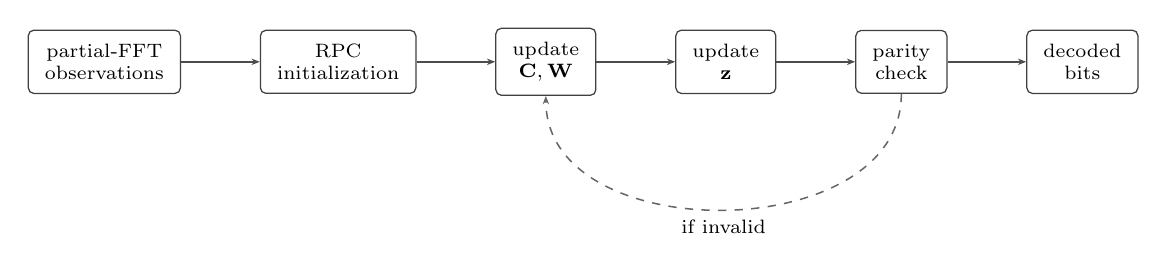
\begin{tikzpicture}[node distance=10mm]
			\node[mbox] (obs) {partial-FFT\\observations};
			\node[mbox, right=of obs] (init) {RPC\\initialization};
			\node[mbox, right=of init] (model) {update\\$\mathbf C,\mathbf W$};
			\node[mbox, right=of model] (bits) {update\\$\mathbf z$};
			\node[mbox, right=of bits] (check) {parity\\check};
			\node[mbox, right=of check] (dec) {decoded\\bits};
			\draw[marr] (obs) -- (init);
			\draw[marr] (init) -- (model);
			\draw[marr] (model) -- (bits);
			\draw[marr] (bits) -- (check);
			\draw[marr] (check) -- (dec);
			\draw[mloop] (check.south) to[out=-90,in=-90,looseness=1.1]
			node[below,font=\scriptsize] {if invalid} (model.south);
		\end{tikzpicture}
		\caption{Minimal JUNA inference loop. RPC provides the pilot-trained initialization; subsequent iterations alternate front-end and bit-latent updates until a valid parity check or the iteration budget is reached.}
		\label{fig:juna-pipeline}
	\end{figure}
	
	
	Objective~\eqref{eq:juna_total} is nonconvex because the branch coefficients \(\mathbf C\), combiners \(\mathbf W\), and bit latents \(\mathbf z\) are coupled through \(s_k(\mathbf z)\), the branch-domain forward model, and the parity products. The solver therefore does not claim global optimality. It exploits the block structure so that front-end refinement and code-constrained bit refinement support one another throughout the solve rather than acting as separate processing stages (Figure~\ref{fig:juna-pipeline}).
	
	The blocks have different numerical character. For fixed \(\mathbf z\), the update of \(\mathbf C\) is a ridge-regularized least-squares problem. For fixed \((\mathbf C,\mathbf z)\), the update of each \(\mathbf w_k\) is also ridge-regularized least squares. The \(\mathbf z\)-block is smooth but nonconvex due to the QPSK map and parity products; gradient or quasi-Newton steps are therefore used as local refinement rather than as a guarantee of global optimality.
	
	\subsection{Soft-Symbol-Model Update}
	
	Given current latents \(\mathbf z^{(t)}\), define \(s_k^{(t)}=s_k(\mathbf z^{(t)})\). The front-end subproblem updates \((\mathbf C,\mathbf W)\) by minimizing the terms of~\eqref{eq:juna_total} that depend on the branch model and scalar combiners:
	\begin{equation}
		\begin{aligned}
			\min_{\mathbf C,\mathbf W}\quad
			&\lambda_{\mathrm d}
			\sum_{k\in\mathcal K}
			\left\|
			\mathbf Y_k-
			\sum_{q\in\mathcal B_K(k)}\mathbf c_{k,q}s_q^{(t)}
			\right\|_{\Sigma_k^{-1}}^2
			+\eta\sum_{p\in\mathcal P}|\mathbf w_p^H\mathbf Y_p-P_p|^2
			\\
			&+\rho\sum_{k\in\mathcal D}|\mathbf w_k^H\mathbf Y_k-s_k^{(t)}|^2
			+\gamma_C\|\mathbf C\|_F^2
			+\gamma_W\sum_k\|\mathbf w_k\|_2^2
			+\gamma_S\sum_k\|\mathbf w_{k+1}-\mathbf w_k\|_2^2 .
		\end{aligned}
		\label{eq:frontend_subproblem_juna}
	\end{equation}
	Without the data-symbol and smoothness terms, the \(\mathbf w_k\) update reduces to the same pilot-trained ridge system as RPC. Thus RPC is both the strongest separate RPC-and-decoding baseline and a practical initializer/inner block for the joint solver.
	
	For the branch coefficients, define
	\[
	\mathbf E_k
	=\mathbf Y_k-\sum_{q\in\mathcal B_K(k)}\mathbf c_{k,q}s_q^{(t)} .
	\]
	The resulting \(\mathbf C\)-block is linear least squares with ridge regularization. If additional nonlinear nonideality parameters are included, the same term remains differentiable and can be updated by Wirtinger-gradient steps; the linear banded model is the cleanest version for the current paper.
	
	\subsection{Latent-Bit Update}
	
	With \((\mathbf C,\mathbf W)\) fixed, JUNA updates the bit latents by
	\begin{equation}
		\begin{aligned}
			\min_{\mathbf z}\quad
			&\lambda_{\mathrm d}
			\sum_{k\in\mathcal K}
			\left\|
			\mathbf Y_k-
			\sum_{q\in\mathcal B_K(k)}\mathbf c_{k,q}s_q(\mathbf z)
			\right\|_{\Sigma_k^{-1}}^2
			+\rho\sum_{k\in\mathcal D}|\mathbf w_k^H\mathbf Y_k-s_k(\mathbf z)|^2
			\\
			&+\lambda_{\mathrm p}
			\sum_{j=1}^{m}
			\left(1-\prod_{i\in\mathcal N_j}\xi_i(\mathbf z)\right)^2 .
		\end{aligned}
		\label{eq:z_subproblem_juna}
	\end{equation}
	This block is naturally handled by automatic differentiation because \(\mathbf z\mapsto\xi_i(\mathbf z)\mapsto s_k(\mathbf z)\) is nonlinear even before the parity products are added. The explicit bit-level notation is important: the parity check acts on \(\xi_i\), while the OFDM observation model acts on the complex QPSK symbols \(s_k\).
	
	\subsection{Initialization and Stopping}
	
	Because the objective is nonconvex, initialization matters. A natural choice is to seed the soft-symbol model from pilot-trained RPC: initialize \(\mathbf{W}^{(0)}\) from pilot-weighted ridge least squares (or an RLS pass), initialize \(\mathbf{C}^{(0)}\) from a neutral low-order local model, form \(\widetilde{s}_k^{(0)}=(\mathbf w_k^{(0)})^{H}\mathbf Y_k\), demap these scalar soft symbols to initial bit latents \(\mathbf z^{(0)}\), and then construct \(s_k(\mathbf z^{(0)})\) through~\eqref{eq:qpsk_soft_symbol_from_bits}. The joint solver thus starts from a meaningful pilot-trained model before code-coupled iterations begin, and its first outer iteration remains anchored to RPC behavior.
	
	The solver terminates on any of: a valid decode (the most meaningful criterion, as in DFEC), a stalled parity residual, total-loss decrease below a threshold, or exhaustion of the outer-iteration budget.
	
	\begin{figure}[tbp]
		\centering
		\begin{minipage}{0.9\textwidth}
			\small
			\textbf{Algorithm 5.1: Hybrid JUNA solver}
			
			\begin{enumerate}
				\item \textbf{Input:} partial-FFT observations \(\{\mathbf{Y}_k\}\), pilot set \(\mathcal{P}\), pilot symbols \(\{X_p\}_{p\in\mathcal{P}}\), parity-check matrix \(\mathbf{P}\), weights \((\lambda_{\mathrm d},\eta,\rho,\gamma_C,\gamma_W,\gamma_S,\lambda_{\mathrm p})\), and maximum outer iterations \(T_{\max}\).
				\item Initialize \(\mathbf{W}^{(0)}\) from pilot-trained RPC, \(\mathbf{C}^{(0)}\) from a neutral local model, and \(\mathbf{z}^{(0)}\) from the initial pre-decoder soft symbols.
				\item For \(t=0,1,\dots,T_{\max}-1\):
				\begin{enumerate}
					\item update \(\mathbf{W}^{(t+1)}\) by a soft-symbol-model ridge/least-squares step.
					\item update \(\mathbf{C}^{(t+1)}\) by one or more manual-gradient steps.
					\item update \(\mathbf{z}^{(t+1)}\) by one or more AD-based gradient steps.
					\item form hard bit decisions from \(\xi_i(\mathbf z^{(t+1)})\) and QPSK symbols from \(s_k(\mathbf z^{(t+1)})\); stop if all parity checks are satisfied.
				\end{enumerate}
				\item \textbf{Return:} decoded bits and final soft-symbol-model estimates.
			\end{enumerate}
		\end{minipage}
		\caption{Hybrid JUNA solver.}
		\label{fig:juna_algorithm}
	\end{figure}

%	\section{Information-Theoretic View of the RPC--JUNA Separation}
%	\label{ssec:info_theoretic_juna_rpc}
%	
%	The preceding construction can also be interpreted as a reduction of receiver-side
%	information loss. This interpretation is useful because JUNA does not change the
%	physical channel capacity: the received waveform contains the same information regardless
%	of the receiver. The distinction is that a modular RPC receiver compresses the partial-FFT
%	observations into scalar pre-decoder statistics before the LDPC constraints are used,
%	whereas JUNA keeps the Doppler/ICI observation model and the code constraints coupled
%	during inference.
%	
%	Let \(\mathbf b\in\mathcal C\) denote the coded bit vector, where
%	\begin{equation}
%		\mathcal C
%		=
%		\{\mathbf b\in\F_2^{n_b}:\mathbf P\mathbf b^T=\mathbf 0\}
%	\end{equation}
%	is the LDPC codebook. Let
%	\[
%	\mathbf Y=\{\mathbf Y_k:k\in\mathcal K\}
%	\]
%	denote the collection of partial-FFT observations. Under residual Doppler, the
%	branch-domain likelihood is not carrierwise diagonal. In the local banded model,
%	\begin{equation}
%		\mathbf Y_k
%		=
%		\sum_{q\in\mathcal B_K(k)}
%		\mathbf c_{k,q}s_q(\mathbf b)
%		+
%		\mathbf n_k,
%		\qquad
%		\mathbf n_k\sim\mathcal{CN}(\mathbf 0,\Sigma_k).
%		\label{eq:info_branch_likelihood}
%	\end{equation}
%	Consequently the likelihood of a received carrier depends on a neighborhood of
%	transmitted coded symbols rather than only on the symbol occupying the same carrier:
%	\begin{equation}
%		p(\mathbf Y\mid \mathbf b,\mathbf C)
%		=
%		\prod_{k\in\mathcal K}
%		p\!\left(
%		\mathbf Y_k
%		\mid
%		\{s_q(\mathbf b):q\in\mathcal B_K(k)\},
%		\mathbf C
%		\right).
%		\label{eq:coupled_likelihood}
%	\end{equation}
%	This is the essential difference from the diagonal OFDM model. Once residual Doppler
%	has created local ICI, the relevant receiver statistic is generally not a scalar
%	per carrier; it is a local observation pattern involving neighboring coded symbols and
%	the branch-domain nonideality coefficients.
%	
%	The RPC receiver forms scalar pre-decoder symbols
%	\begin{equation}
%		\widetilde X_k
%		=
%		\widehat{\mathbf W}_k^H\mathbf Y_k,
%		\qquad
%		\widetilde{\mathbf X}
%		=
%		\{\widetilde X_k:k\in\mathcal K\},
%		\label{eq:rpc_scalar_statistic_info}
%	\end{equation}
%	where \(\widehat{\mathbf W}_k\) is trained from pilots, or from pilot-anchored recursive
%	updates, before LDPC decoding is performed. Thus the modular receiver induces the
%	conditional Markov chain
%	\begin{equation}
%		\mathbf b
%		\longrightarrow
%		\mathbf Y
%		\longrightarrow
%		\widetilde{\mathbf X}
%		\qquad
%		\text{given the pilot pattern and receiver side information}.
%		\label{eq:rpc_markov_chain}
%	\end{equation}
%	By the data-processing inequality,
%	\begin{equation}
%		I(\mathbf b;\widetilde{\mathbf X})
%		\le
%		I(\mathbf b;\mathbf Y).
%		\label{eq:rpc_dpi}
%	\end{equation}
%	The inequality itself does not imply that RPC is poor. It only states that the scalar
%	RPC statistic cannot contain more information about the coded word than the original
%	partial-FFT observations. RPC is information-lossless only when
%	\(\widetilde{\mathbf X}\) is sufficient for \(\mathbf b\) with respect to \(\mathbf Y\),
%	i.e.,
%	\begin{equation}
%		p(\mathbf b\mid \mathbf Y)
%		=
%		p(\mathbf b\mid \widetilde{\mathbf X}).
%		\label{eq:sufficiency_condition_rpc}
%	\end{equation}
%	Equivalently,
%	\begin{equation}
%		I(\mathbf b;\mathbf Y\mid \widetilde{\mathbf X})=0.
%		\label{eq:conditional_info_zero}
%	\end{equation}
%	In the no-Doppler diagonal regime, a properly equalized scalar statistic per carrier can
%	be close to sufficient because each observation is approximately governed by
%	\(Y_k=H_kX_k+\nu_k\). Under residual Doppler, this condition generally fails. The branch
%	observation \(\mathbf Y_k\) depends on a local neighborhood of coded symbols through
%	\eqref{eq:info_branch_likelihood}, so information about neighboring symbols and local
%	ICI is carried by the vector pattern across partial-FFT branches and adjacent carriers.
%	A scalar statistic \(\widetilde X_k=\widehat{\mathbf W}_k^H\mathbf Y_k\) need not preserve
%	that local information.
%	
%	The meaning of the mutual-information loss can be made explicit by writing
%	\begin{equation}
%		I(\mathbf b;\mathbf Y)
%		=
%		H(\mathbf b)-H(\mathbf b\mid\mathbf Y),
%		\qquad
%		I(\mathbf b;\widetilde{\mathbf X})
%		=
%		H(\mathbf b)-H(\mathbf b\mid\widetilde{\mathbf X}).
%		\label{eq:mi_entropy_definitions}
%	\end{equation}
%	Thus \(I(\mathbf b;\mathbf Y)\) measures the reduction in uncertainty about the coded
%	word provided by the full partial-FFT observation, while
%	\(I(\mathbf b;\widetilde{\mathbf X})\) measures the reduction that remains after RPC
%	has compressed those observations into scalar pre-decoder symbols. Since
%	\(\widetilde{\mathbf X}=g(\mathbf Y)\) is a deterministic receiver statistic computed
%	from \(\mathbf Y\), the residual information discarded by RPC is
%	\begin{equation}
%		I(\mathbf b;\mathbf Y\mid\widetilde{\mathbf X})
%		=
%		H(\mathbf b\mid\widetilde{\mathbf X})
%		-
%		H(\mathbf b\mid\mathbf Y).
%		\label{eq:residual_information_rpc}
%	\end{equation}
%	The identity follows because
%	\(H(\mathbf b\mid\mathbf Y,\widetilde{\mathbf X})=H(\mathbf b\mid\mathbf Y)\) whenever
%	\(\widetilde{\mathbf X}\) is a function of \(\mathbf Y\). Equation
%	\eqref{eq:residual_information_rpc} is the bottleneck term: it is the information about
%	the coded word that remains in the partial-FFT observations after the RPC scalar output
%	is already known. In a diagonal channel this term can be small. In a Doppler-distorted
%	channel it can be significant, because the discarded branch structure contains information
%	about local ICI and neighboring coded symbols.
%	
%	A two-branch toy model makes the loss visible. Suppose
%	\begin{equation}
%		\mathbf Y_k
%		=
%		x_k
%		\begin{bmatrix}1\\1\end{bmatrix}
%		+
%		\alpha x_{k+1}
%		\begin{bmatrix}1\\-1\end{bmatrix}
%		+
%		\mathbf n ,
%		\label{eq:toy_branch_model_info}
%	\end{equation}
%	with \(x_k,x_{k+1}\in\{\pm1\}\). If the RPC statistic is the branch average,
%	\begin{equation}
%		\widetilde X_k
%		=
%		\frac{Y_{k,1}+Y_{k,2}}{2},
%		\label{eq:toy_rpc_average}
%	\end{equation}
%	then, in the noiseless case, \(\widetilde X_k=x_k\), while the branch difference
%	\begin{equation}
%		\frac{Y_{k,1}-Y_{k,2}}{2}
%		=
%		\alpha x_{k+1}
%		\label{eq:toy_branch_difference}
%	\end{equation}
%	contains information about the neighboring symbol. Thus the full branch vector carries
%	information about the local pair \((x_k,x_{k+1})\), whereas the scalar RPC statistic
%	does not. In this example,
%	\begin{equation}
%		I\big((x_k,x_{k+1});\mathbf Y_k\big)
%		>
%		I\big((x_k,x_{k+1});\widetilde X_k\big)
%	\end{equation}
%	whenever \(\alpha\neq0\) and the observation noise is not overwhelming. This is the
%	operational meaning of \(I(\mathbf b;\mathbf Y\mid\widetilde{\mathbf X})>0\).
%	
%	The same point can be stated as a decoding-metric mismatch. After scalarization, the
%	LDPC decoder is typically supplied with a metric of the form
%	\begin{equation}
%		q_{\mathrm{RPC}}(\widetilde{\mathbf X}\mid\mathbf b)
%		=
%		\prod_{k\in\mathcal D}
%		q_k(\widetilde X_k\mid s_k(\mathbf b)),
%		\label{eq:rpc_factorized_metric}
%	\end{equation}
%	which treats the pre-decoder observations as approximately carrierwise independent.
%	The true residual-Doppler likelihood, by contrast, has the coupled form
%	\eqref{eq:coupled_likelihood}. The discrepancy between
%	\eqref{eq:rpc_factorized_metric} and \eqref{eq:coupled_likelihood} is not merely a
%	parametric error; it changes the information made available to the decoder. Structured
%	ICI generated by neighboring coded symbols is partly represented as effective noise.
%	
%	JUNA reduces this separation loss by retaining the coupled likelihood during
%	code-constrained inference. Its objective may be viewed as a regularized approximate
%	negative log-posterior for
%	\[
%	p(\mathbf b,\mathbf C,\mathbf W\mid \mathbf Y,\mathcal I),
%	\]
%	where \(\mathcal I\) denotes pilots, noise statistics, and receiver side information.
%	In the hard-symbol idealization, the corresponding joint MAP problem is
%	\begin{equation}
%		(\widehat{\mathbf b},\widehat{\mathbf C},\widehat{\mathbf W})
%		\approx
%		\arg\max_{\mathbf b\in\mathcal C,\mathbf C,\mathbf W}
%		p(\mathbf Y\mid \mathbf b,\mathbf C)
%		p(\mathbf C,\mathbf W\mid\mathcal I).
%		\label{eq:juna_joint_map_info}
%	\end{equation}
%	The relaxed JUNA objective in \eqref{eq:juna_total} implements a differentiable surrogate
%	of this problem: the observation-consistency term represents the coupled
%	Doppler/ICI likelihood, the pilot term anchors known symbols, the combiner-symbol term
%	links scalar soft outputs to the relaxed QPSK field, and the parity penalty introduces
%	the LDPC code structure during front-end refinement.
%	
%	The consequence is that reliable coded data symbols can act as soft pilots. In a modular
%	receiver, only the explicit pilot set \(\mathcal P\) constrains the front-end coefficients
%	before decoding. In JUNA, the code constraints can make some data symbols highly reliable
%	during inference; those symbols then provide additional soft constraints on
%	\(\mathbf C\) and \(\mathbf W\). In entropy terms, the intended effect is
%	\begin{equation}
%		H(\mathbf C,\mathbf W\mid \mathbf Y,\mathcal P,\mathcal C)
%		\le
%		H(\mathbf C,\mathbf W\mid \mathbf Y,\mathcal P),
%		\label{eq:frontend_entropy_reduction}
%	\end{equation}
%	with strict reduction whenever the code constraints resolve ambiguity that is not resolved
%	by pilots alone. Improved front-end certainty then improves the reliability of the bit
%	likelihoods supplied to the decoder.
%	
%	A minimal two-symbol example illustrates the same mechanism at the symbol level. Suppose
%	\begin{align}
%		y_1 &= x_1+\alpha x_2+n_1,\\
%		y_2 &= \alpha x_1+x_2+n_2,
%	\end{align}
%	with \(x_1,x_2\in\{\pm1\}\). If \(x_2\) is unknown and the receiver does not use any
%	constraint linking it to \(x_1\), the term \(\alpha x_2\) is effective interference in
%	the first observation. If the code implies \(x_1=x_2\), then
%	\begin{align}
%		y_1 &= (1+\alpha)x_1+n_1,\\
%		y_2 &= (1+\alpha)x_1+n_2.
%	\end{align}
%	The same coupling term that appears as interference to a separated front end becomes
%	coherent information once the code constraint is used during inference. This is the
%	basic information-theoretic reason to couple Doppler/ICI estimation and code-constrained
%	detection.
%	
%	The resulting claim is therefore not that JUNA increases the channel capacity, but that
%	it uses a better receiver statistic and a better matched decoding metric. Whenever the
%	RPC statistic \(\widetilde{\mathbf X}\) is not sufficient for \(\mathbf b\), and whenever
%	the JUNA likelihood model better approximates the coupled residual-Doppler channel than
%	the factorized RPC metric, the generalized achievable rate of the JUNA metric can exceed
%	that of RPC followed by LDPC decoding. Equivalently, JUNA can reduce posterior uncertainty
%	by avoiding the replacement
%	\[
%	\mathbf Y\mapsto\widetilde{\mathbf X}
%	\]
%	before the code constraints are used. Under residual Doppler, the residual term
%	\[
%	I(\mathbf b;\mathbf Y\mid\widetilde{\mathbf X})
%	\]
%	is precisely the branch/local-ICI information that a scalar modular receiver can compress
%	away, and that a coupled JUNA receiver is designed to exploit.
%
%	
%	The claim of Section~\ref{chap:juna} is that JUNA's advantage over separate RPC and decoding grows with the dynamic non-diagonality of the channel. We test that claim in two complementary ways. First, we use the deterministic six-tap underwater acoustic channel used in the RPC literature, which gives an apple-to-apple comparison against the strongest separate RPC-and-decoding baseline. Second, we evaluate \(60\) realistic channels with different delay spreads, boundary conditions, and frequency-selective acoustic paths.
		\section{Validation}
	\label{chap:results}

	The architectural claim of Section~\ref{chap:juna} is sharper than ``JUNA reduces BER''. It says JUNA's advantage \emph{tracks the dynamic non-diagonality of the channel} --- large where the residual operator carries heavy off-diagonal energy, small where it does not. That is a statement about which channels benefit, not about how much a single channel improves, and no single SNR sweep can falsify it.

	We therefore validate JUNA along two complementary axes. A single-channel SNR sweep on the deterministic six-tap underwater multipath channel used in the RPC literature (Section~\ref{ssec:fixed_channel}) pins down an apple-to-apple comparison on the same benchmark against which the strongest separate-decoder baseline was originally evaluated. A population study across 60 realistic shallow-water geometries (Section~\ref{ssec:pekeris}) then tests the architectural prediction directly: do channels with large mean ICI ratio produce the largest RPC/JUNA gains, do channels with little dynamic non-diagonality produce small gains, and does the spread of gains across the cohort match the argument? One study guards against the obvious objection that the result is an artefact of cohort choice; the other tests the prediction the theory actually makes. Both share the packet-level harness described next.

	\subsection{Simulation Framework}
	\label{ssec:simframework}

	The packet-level harness is shared between both studies. Each trial runs a complete packet through waveform generation, channel distortion, standard Doppler generation, packet acquisition, partial-FFT observation formation, branch-specific inference, and LDPC-coded error counting.
	
	\subsubsection{Six-Tap Baseline Channel}
	
	The deterministic baseline used for the fixed-channel sweep is the six-tap underwater multipath channel in Table~\ref{tab:paper_channel_taps}. This channel is presented first because the RPC reference also uses this style of six-tap underwater acoustic benchmark; keeping it lets us make an apple-to-apple comparison between RPC and JUNA before moving to a larger set of realistic channel geometries. With tap delays \(\{d_\ell\}\), powers \(\{p_\ell\}\), and fixed phases \(\{\phi_\ell\}\),
	\begin{equation}
		h[n]
		=
		\sum_{\ell=0}^{5}
		\sqrt{p_\ell}\, e^{j\phi_\ell}\,\delta[n-d_\ell],
		\qquad
		H_k
		=
		\sum_{\ell=0}^{5}
		\sqrt{p_\ell}\, e^{j\phi_\ell} e^{-j2\pi k d_\ell/N}.
		\label{eq:sim_H_from_taps}
	\end{equation}
	
	\begin{table}[H]
		\centering
		\caption{Deterministic six-tap baseline channel used in the fixed-channel benchmark.}
		\label{tab:paper_channel_taps}
		\begin{tabular}{cccc}
			\toprule
			Tap index & Delay (ms) & Power (dB) & Default phase (rad) \\
			\midrule
			0 & 0.0 & 0.0 & 0.0 \\
			1 & 0.8 & -0.9 & 0.7 \\
			2 & 1.7 & -4.9 & -1.1 \\
			3 & 2.7 & -8.0 & 2.0 \\
			4 & 3.8 & -7.8 & -2.4 \\
			5 & 5.0 & -23.7 & 1.3 \\
			\bottomrule
		\end{tabular}
	\end{table}
	
	The realistic-channel study then replaces the deterministic taps with impulse responses generated from shallow-water acoustic geometry. The Pekeris model is used here as the propagation method that converts channel parameters --- range, bathymetry, transmitter/receiver depths, and boundary conditions --- into a channel impulse response. These geometries are a better proxy for real underwater links because they produce a spread of notches, delay tails, and Doppler-induced ICI patterns that a single six-tap channel cannot cover.
	
	\subsubsection{Simulation Procedure}
	
	\begin{figure}[H]
		\centering
		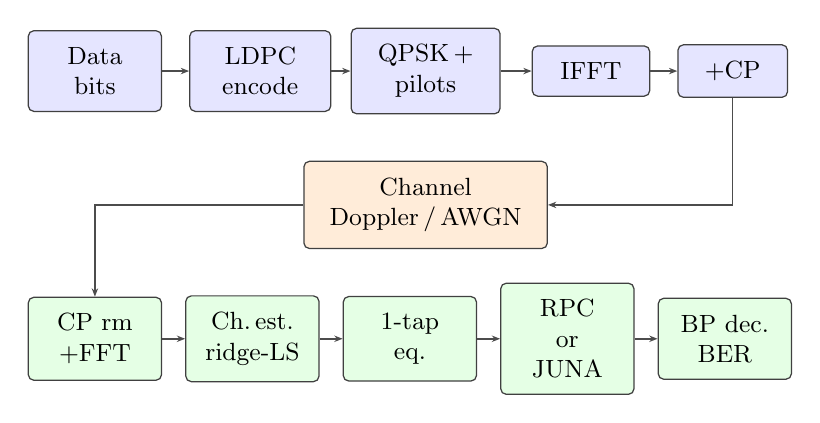
\begin{tikzpicture}[font=\footnotesize]
			% TX Row (top, y=0)
			\node[simbox,fill=blue!10,text width=1.2cm] at (0,0)    (data)   {Data\\bits};
			\node[simbox,fill=blue!10,text width=1.3cm] at (2.1,0)  (enc)    {LDPC\\encode};
			\node[simbox,fill=blue!10,text width=1.4cm] at (4.2,0)  (pilots) {QPSK\,+\\pilots};
			\node[simbox,fill=blue!10,text width=1.0cm] at (6.3,0)  (ifft)   {IFFT};
			\node[simbox,fill=blue!10,text width=0.9cm] at (8.1,0)  (cp)     {+CP};

			% Channel Row (middle, y=-1.7)
			\node[simbox,fill=orange!15,text width=2.6cm] at (4.2,-1.7) (chan) {Channel\\Doppler\,/\,AWGN};

			% RX Row (bottom, y=-3.4)
			\node[simbox,fill=green!10,text width=1.2cm] at (0,-3.4)   (cprm) {CP rm\\+FFT};
			\node[simbox,fill=green!10,text width=1.2cm] at (2.0,-3.4) (hest) {Ch.\,est.\\ridge-LS};
			\node[simbox,fill=green!10,text width=1.2cm] at (4.0,-3.4) (eq)   {1-tap\\eq.};
			\node[simbox,fill=green!10,text width=1.2cm] at (6.0,-3.4) (rx)   {RPC\\or\\JUNA};
			\node[simbox,fill=green!10,text width=1.2cm] at (8.0,-3.4) (ber)  {BP dec.\\BER};

			% TX arrows (left to right)
			\draw[marr] (data)   -- (enc);
			\draw[marr] (enc)    -- (pilots);
			\draw[marr] (pilots) -- (ifft);
			\draw[marr] (ifft)   -- (cp);

			% TX -> Channel (down + left)
			\draw[marr] (cp.south) |- (chan.east);

			% Channel -> RX (down + left)
			\draw[marr] (chan.west) -| (cprm.north);

			% RX arrows (left to right)
			\draw[marr] (cprm) -- (hest);
			\draw[marr] (hest) -- (eq);
			\draw[marr] (eq)   -- (rx);
			\draw[marr] (rx)   -- (ber);
		\end{tikzpicture}
		\caption{Packet-level simulation flow. Data bits are LDPC-encoded, mapped with pilots, converted to CP-OFDM via IFFT, passed through the channel with Doppler and AWGN, then processed by CP removal, pilot ridge-LS channel estimation, one-tap equalization, reception (RPC/JUNA), and BP decoding for BER counting.}
		\label{fig:simulation_flow}
	\end{figure}
	
	One trial proceeds as follows: sample data bits, LDPC-encode them, map QPSK data and pilots onto \(N=2048\) subcarriers, apply the IFFT and a \(256\)-sample CP, pass the packet through the underlying channel and standard Doppler generation, remove the CP after acquisition and Doppler compensation, form the full-FFT and \(P=4|8|16|32\) partial-FFT observations, estimate the diagonal channel from pilots using ridge LS, apply one-tap equalization using the estimated channel, run the receiver under test (RPC, or JUNA), and produce hard/soft decisions for BP decoding and error counting. At each SNR, trials repeat until every method accumulates at least 10 coded bit errors or a packet budget is reached. Reported BER is computed from true packet counts via
	\begin{equation}
		\mathrm{BER}_m
		=
		\frac{\sum_{q=1}^{Q} e_m^{(q)}}{\sum_{q=1}^{Q} n_m^{(q)}},
		\label{eq:packet_ber_aggregate}
	\end{equation}
	where \(e_m^{(q)}\) and \(n_m^{(q)}\) are the coded bit errors and coded bits counted for method \(m\) on packet \(q\), and \(Q\) is the total number of packets processed at that SNR.
	
	\subsubsection{Packet and Coding Setup}
	
	Each packet is a QPSK payload using \(N=2048\), CP length \(256\), sampling rate \(f_s=12\) kHz, carrier spacing \(\Delta f=f_s/N=5.859375\) Hz, and pilot ratio \(0.25\). At the receiver the packet is distorted by the channel and processed by a coarse-to-fine acquisition that searches over delay and Doppler scale via preamble correlation; after alignment, CP removal, and AWGN addition, the resulting block \(y_{\mathrm{blk}}[n]\) yields
	\begin{align}
		Y_k^{\mathrm{full}}
		&=
		\frac{1}{\sqrt{N}}
		\sum_{n=0}^{N-1}
		y_{\mathrm{blk}}[n] e^{-j2\pi kn/N},
		&
		\mathbf{Y}_k
		&=
		\texttt{partial\_ffts}(y_{\mathrm{blk}},P).
		\label{eq:sim_observation_generation}
	\end{align}
	The diagonal channel used by the one-tap equalizer is estimated from the pilot carriers by a time-domain ridge least-squares fit. Let \(p_r\in\mathcal{P}\) denote the pilot-carrier indices and choose
	\[
		L_h=\min\{N_{\mathrm{cp}}+1,\max(8,|\mathcal P|)\},
		\qquad
		\rho_{\mathrm{LS}}=10^{-3}.
	\]
	With
	\[
		A_{r\ell}=X_{p_r}e^{-j2\pi p_r\ell/N},
		\qquad
		\ell=0,\ldots,L_h-1,
	\]
	the estimator solves
	\begin{equation}
		\widehat{\mathbf h}
		=
		\arg\min_{\mathbf h\in\mathbb C^{L_h}}
		\sum_{p_r\in\mathcal P}
		\left|Y_{p_r}^{\mathrm{full}}-\sum_{\ell=0}^{L_h-1}A_{r\ell}h_\ell\right|^2
		+\rho_{\mathrm{LS}}\|\mathbf h\|_2^2
		=
		(A^{H}A+\rho_{\mathrm{LS}}I)^{-1}A^{H}\mathbf y_{\mathcal P}.
		\label{eq:pilot_ridge_ls}
	\end{equation}
	The frequency response \(\widehat H_k\) is obtained by zero-padding \(\widehat{\mathbf h}\) to length \(N\) and applying an \(N\)-point FFT. The one-tap equalized observation is then
	\begin{equation}
		\widehat X_k
		=
		\frac{\widehat H_k^{*}}{|\widehat H_k|^2+\sigma^2}\,
		Y_k^{\mathrm{full}},
		\label{eq:estimated_channel_equalizer}
	\end{equation}
	and the same pilot-estimated channel is used to initialize the separate RPC-and-decoding path and JUNA. For the uniform comb pilot pattern, the implementation evaluates~\eqref{eq:pilot_ridge_ls} with the equivalent FFT-diagonalized computation, which gives the same ridge-LS estimate without forming \(A\) explicitly.
	
	The coded benchmark uses a rate-\(1/2\) LDPC code with BP decoder. The same parity-check matrix is exposed to JUNA via its code penalty, so the joint and post-receiver decoders are tested under identical packet coding assumptions. Table~\ref{tab:benchmark_scenario_defaults} lists the remaining parameters.
	
	\begin{table}[tbp]
		\centering
		\caption{Default packet-level benchmark configuration used in the comparison study.}
		\label{tab:benchmark_scenario_defaults}
		\begin{tabular}{p{0.34\linewidth}p{0.60\linewidth}}
			\toprule
			Item & Value \\
			\midrule
			OFDM size \(N\) & \(2048\) \\
			Cyclic prefix & \(256\) samples \\
			Pilot-LS channel length \(L_h\) & Automatic, \(L_h=\min\{N_{\mathrm{cp}}+1,\max(8,|\mathcal P|)\}\) \\
			Partial-FFT branches \(P\) & \(32\) \\
			Pilot ratio & \(0.20\) \\
			Sampling rate / carrier spacing & \(12\) kHz / \(5.859375\) Hz \\
			FEC & Rate-\(1/2\) LDPC code with BP decoder. \\
			Stopping rule & minimum \(10\) coded errors or maximum \(1000\) packets per SNR \\
			RPC parameters & \(\lambda=0.998\), \(\delta=5\), \(\alpha=0.05\) \\
			JUNA defaults & \(300\) iterations, \(4\) subbands, \(K_{\mathrm{ICI}}=2\), pilot-LS init for \(\mathbf{W}\), delta init for \(\mathbf{C}\), \(\lambda_{\mathrm{pil}}=\lambda_{\mathrm{dat}}=\lambda_{\mathrm{code}}=1\), \(\lambda_{\mathrm{const}}=0.25\), demixing enabled \\
			\bottomrule
		\end{tabular}
	\end{table}
	
	\subsection{Packet-Level Verification on the Baseline Channel}
	\label{ssec:fixed_channel}

	Before turning to the population study, we verify on the deterministic six-tap baseline of Table~\ref{tab:paper_channel_taps} that JUNA actually delivers a coded-BER advantage over separate RPC-and-BP on a single channel. This is the apple-to-apple comparison: the same six-tap underwater multipath channel against which the RPC literature is benchmarked, run end-to-end through the packet-level harness of Section~\ref{ssec:simframework}.

	The executed run used SNR \(0{:}2{:}10\) dB, standard Doppler generation with draws \(a\sim\mathrm{Uniform}[-1.5\times 10^{-4},\,1.5\times 10^{-4}]\), and the stopping rule ``min \(10\) coded errors per method or max \(300\) packets per SNR.'' The 0, 2, 4, and 6 dB points completed during the run (with completed packet counts \(1\), \(1\), \(4\), and \(26\) respectively); the directly observed values are plotted in Figure~\ref{fig:tuicoded_ber_curve}. JUNA outperforms separate RPC and BP decoding over the completed low-to-mid SNR points, with the separation growing from 4\,dB onward. This is the single-channel pattern that the 60-channel population study below extends to a much wider range of operating conditions.

	\begin{figure}[tbp]
		\centering
		\includegraphics[width=0.82\textwidth]{figs/coded_sweep_curve.pdf}
		\caption{Coded BER versus SNR from the directly observed completed points of the executed packet-level sweep on the deterministic six-tap baseline channel.}
		\label{fig:tuicoded_ber_curve}
	\end{figure}

	
\subsection{Realistic Channel Geometry Study}
\label{ssec:pekeris}

One SNR sweep on one channel is not enough. The architectural argument of Section~\ref{chap:juna} predicts \emph{which} channels should benefit most from JUNA --- those where residual Doppler creates strong carrier-to-carrier mixing --- and a claim of that shape only becomes testable across an ensemble. So we sweep 60 shallow-water geometries instead of one.

The geometries vary along four axes: range (100--500\,m), bathymetry (20--50\,m), transmitter and receiver depths (5--15\,m), and the bottom and surface boundary types (fluid, rigid, pressure-release, windy). Each combination is fed through a Pekeris propagation model, and the impulse response that comes out is used by the simulation flow of Section~\ref{ssec:fixed_channel}. The full configuration list is long; it lives in the appendix as Table~\ref{tab:cohort}, where the channels are renumbered 1--60 in ascending library order so the BER figures can use compact IDs.

The rest of the subsection looks at this ensemble through three views at increasing zoom. The error-floor histogram (Fig.~\ref{fig:error-floor-histogram}) gives the ensemble view. Five landmark channels (Table~\ref{tab:selected_channels} and Fig.~\ref{fig:five-rows}) tie that ensemble shift to specific geometries. A pilot-ratio sweep on one channel (Fig.~\ref{fig:profile020_stem_bundle}) then exposes the rescue mechanism behind the shift.

\subsubsection{Ensemble shift: error-floor histogram}

Figure~\ref{fig:error-floor-histogram} compresses the 60-channel ensemble into a one-dimensional view. The horizontal axis is the error-floor BER, binned in units of \(10^{-4}\). The vertical axis counts how many channels fall into each bin. Each bin contains two side-by-side bars: a red one for separate RPC\(\to\)BP decoding, a blue one for JUNA.

\begin{figure}[tbp]
	\centering
	\includegraphics[width=0.95\linewidth]{figs/error_floor_histogram_rpc_yuna_20-120.pdf}
	\caption{\textbf{Grouped histogram of error-floor BER for the reference 60-channel ensemble.} Horizontal axis: error-floor BER, binned in units of $10^{-4}$. Vertical axis: number of channels (out of 60) whose error floor falls in each bin. Each bin contains two side-by-side bars; the red one counts channels under separate RPC$\to$BP decoding and the blue one counts channels under JUNA. JUNA mass is concentrated on the left (lower BER), RPC mass on the right (higher BER) --- the same advantage that the per-channel rows resolve case by case.}
	\label{fig:error-floor-histogram}
\end{figure}

Sweeping left to right, the JUNA bars dominate the low-BER bins, the two methods overlap in the middle, and the RPC bars take over the high-BER tail. The whole distribution shifts. So JUNA's advantage is not a handful of friendly geometries --- it is a property of the cohort as a whole.

\subsubsection{Five landmark channels}

The histogram says the ensemble shifts; it does not say which geometries drive that shift. Table~\ref{tab:selected_channels} picks five landmark channels that span the corners of the cloud, and Figure~\ref{fig:five-rows} unfolds each one into a four-panel row showing impulse response, static frequency response, and coded BER at \(a=0\) and at \(a=10^{-4}\).

\begin{table}[H]
	\centering
	\scriptsize
	\setlength{\tabcolsep}{2.5pt}
	\begin{tabular}{c l c c c c c}
		\toprule
		ID & Label & Notch (dB) & SFM & $\bar{\eta}$ & BER(JUNA) & Gain RPC/JUNA \\
		\midrule
		42 & flat low-BER gain edge & 11.68 & 0.782 & 0.0202 & $1.21\times10^{-5}$ & 4.09 \\
		20 & high-gain selective edge & 28.64 & 0.707 & 0.0295 & $1.83\times10^{-5}$ & 3.75 \\
		13 & high-gain selective mid-band & 37.08 & 0.594 & 0.0258 & $1.43\times10^{-4}$ & 3.25 \\
		60 & selective weak-tail mid-band & 38.42 & 0.577 & 0.0529 & $1.95\times10^{-4}$ & 1.30 \\
		52 & high-ICI hard floor & 39.67 & 0.559 & 0.1409 & $3.63\times10^{-4}$ & 0.98 \\
		\bottomrule
	\end{tabular}
	\caption{Selected channels from the 60-channel ensemble. BER(JUNA) and gain values are read at the automatically detected error-floor SNR for \(a=10^{-4}\).}
	\label{tab:selected_channels}
\end{table}

Three of the landmarks mark the main regions: an easy low-BER edge (channel 42), a more selective mid-band case (channel 60), and a hard high-ICI floor (channel 52). The other two, channels 20 and 13, sit at the high-gain end of the RPC/JUNA comparison and show that large gains can persist deep into the selective regime. Two summary metrics appear in the table. \emph{Notch depth} is the worst-case max-to-min frequency-response ratio in dB, and \emph{SFM} is the geometric-to-arithmetic mean of the same response; both track static fragility. The \emph{mean ICI ratio} \(\bar{\eta}\) measures how strongly residual Doppler at \(a=10^{-4}\) leaks energy off the diagonal of the OFDM operator, and tracks dynamic leakage.

\begin{figure}[p]
	\centering
	\includegraphics[width=\textwidth,trim=0 0 0 12pt,clip]{figs/profile_095_range200m_bathy30m_tx15m_rx15m_bottom_rigid_surface_windy_bounces_3_fs24000_snr_curve_strict_cpp_yuna_smoothed.png}

	\vspace{0.35em}
	\includegraphics[width=\textwidth,trim=0 0 0 12pt,clip]{figs/profile_049_range400m_bathy30m_tx15m_rx10m_bottom_pressure_release_surface_rigid_bounces_3_fs24000_snr_curve_strict_cpp_yuna_smoothed.png}

	\vspace{0.35em}
	\includegraphics[width=\textwidth,trim=0 0 0 12pt,clip]{figs/profile_038_range500m_bathy30m_tx15m_rx15m_bottom_pressure_release_surface_windy_bounces_3_fs24000_snr_curve_strict_cpp_yuna_smoothed.png}

	\vspace{0.35em}
	\includegraphics[width=\textwidth,trim=0 0 0 12pt,clip]{figs/profile_120_range300m_bathy40m_tx5m_rx5m_bottom_pressure_release_surface_rigid_bounces_3_fs24000_snr_curve_strict_cpp_yuna_smoothed.png}

	\vspace{0.35em}
	\includegraphics[width=\textwidth,trim=0 0 0 12pt,clip]{figs/profile_111_range100m_bathy30m_tx15m_rx10m_bottom_pressure_release_surface_pressure_release_bounces_3_fs24000_snr_curve_strict_cpp_yuna_smoothed.png}
	\caption{\textbf{Five selected channel geometries arranged as a \(5\times4\) panel summary.} Each row shows impulse response, static frequency response, coded BER for \(a=0\), and coded BER for \(a=10^{-4}\). From top to bottom: channel 42 (flat low-BER gain edge), channel 20 (high-gain selective edge), channel 13 (high-gain selective mid-band), channel 60 (selective weak-tail mid-band), and channel 52 (high-ICI hard floor with near-unity RPC/JUNA gain).}
	\label{fig:five-rows}
\end{figure}

The five rows make the histogram shift concrete. Channel 42 is the easy edge: the flattest response of the five, the smallest \(\bar{\eta}\), and the lowest JUNA error floor. Even here, the Doppler panel keeps a visible gap between RPC and JUNA. Channels 20 and 13 push the same high-gain story into more selective territory --- they are notchier than 42, yet their \(\bar{\eta}\) stays modest, and JUNA turns that asymmetry into a sizable BER gain. Channel 60 is harder. The notches stay deep, the JUNA floor lifts, and the gain shrinks. Channel 52 is the hard wall: largest \(\bar{\eta}\) of the five, highest JUNA error floor, and RPC/JUNA ratio close to one. That last point is the useful reminder --- big mean ICI on its own is not enough to guarantee a big gain.

\subsubsection{Pilot-ratio rescue on channel 20}

The histogram and the five landmarks say \emph{what} JUNA improves; the pilot-ratio sweep says \emph{when} that improvement appears. Figure~\ref{fig:profile020_stem_bundle} fixes one channel (channel 1, the first row of Table~\ref{tab:cohort}), holds SNR at \(16\) dB and residual Doppler at \(a=10^{-4}\), and varies the pilot ratio from \(0.05\) to \(0.25\) in steps of \(0.01\).

\begin{figure}[tbp]
	\centering
	\includegraphics[width=0.92\linewidth]{figs/profile020_pilot_ratio_error_floor_stem.pdf}
	\caption{\textbf{Pilot-ratio sweep on channel 1.} Horizontal axis: pilot ratio. Vertical axis: error-floor BER at SNR \(16\) dB and residual Doppler \(a=10^{-4}\), shown on a log scale. The red curve is separate RPC\(\rightarrow\)BP decoding; the blue curve is JUNA. Both methods sit at a high floor for pilot ratios below about \(0.13\), then drop by roughly two orders of magnitude over \(0.13\) to \(0.15\). Above the threshold, JUNA remains consistently below RPC.}
	\label{fig:profile020_stem_bundle}
\end{figure}

The two curves break into three regions. Below pilot ratio \(0.12\), the estimator does not have enough pilots to pin the channel down under residual Doppler; both methods sit at the same high floor near \(10^{-1}\) and adding one more pilot does almost nothing. Between \(0.13\) and \(0.15\) the curves drop by roughly two orders of magnitude. This is the rescue threshold, where pilot support finally overcomes the residual-Doppler ambiguity. Above \(0.15\) both methods plateau, but JUNA's plateau sits roughly half an order of magnitude below RPC's, and that gap holds out to pilot ratio \(0.25\). The ensemble shift seen in the histogram is the distributional consequence of this single-channel rescue: under JUNA most channels sit to the right of their own threshold, while under separate RPC\(\to\)BP a non-trivial fraction still sits to the left.
	
	Table~\ref{tab:cohort} lists the 60 channel geometries used in the study of Section~\ref{chap:results}. Each row specifies range, bathymetry, transmitter and receiver depths, and the bottom/surface boundary conditions used by the acoustic propagation model.
	
	\begin{table}[H]
		\centering
		\scriptsize
		\setlength{\tabcolsep}{2.0pt}
		\renewcommand{\arraystretch}{0.92}
		\caption{Configuration table for the 60 channel geometries. Distances are in meters. Boundary abbreviations: F = fluid, R = rigid, PR = pressure-release, W = windy.}
		\label{tab:cohort}
		\begin{minipage}[t]{0.49\textwidth}
			\vspace{0pt}
			\centering
			\begin{tabular}{@{}rrrrrcc@{}}
				\toprule
				ID & Rng & Bath & Tx & Rx & Bot. & Surf. \\
				\midrule
				1 & 300 & 30 & 10 & 10 & F & PR \\
				2 & 150 & 30 & 10 & 10 & F & PR \\
				3 & 200 & 20 & 10 & 15 & R & R \\
				4 & 100 & 30 & 5 & 10 & F & R \\
				5 & 150 & 30 & 10 & 10 & F & W \\
				6 & 300 & 40 & 10 & 15 & PR & R \\
				7 & 200 & 30 & 5 & 15 & R & R \\
				8 & 500 & 40 & 5 & 15 & F & R \\
				9 & 150 & 30 & 5 & 5 & R & R \\
				10 & 400 & 30 & 15 & 5 & F & W \\
				11 & 400 & 50 & 5 & 5 & F & PR \\
				12 & 500 & 30 & 15 & 15 & R & W \\
				13 & 500 & 30 & 15 & 15 & PR & W \\
				14 & 200 & 30 & 15 & 10 & PR & PR \\
				15 & 500 & 30 & 5 & 5 & F & R \\
				16 & 400 & 30 & 10 & 5 & R & W \\
				17 & 200 & 40 & 5 & 15 & F & PR \\
				18 & 400 & 50 & 15 & 5 & PR & PR \\
				19 & 400 & 30 & 5 & 5 & F & R \\
				20 & 400 & 30 & 15 & 10 & PR & R \\
				21 & 100 & 20 & 5 & 10 & F & R \\
				22 & 150 & 30 & 10 & 10 & R & PR \\
				23 & 400 & 50 & 5 & 5 & R & R \\
				24 & 100 & 30 & 10 & 10 & PR & PR \\
				25 & 300 & 50 & 10 & 10 & R & W \\
				26 & 150 & 40 & 10 & 5 & F & W \\
				27 & 400 & 40 & 15 & 10 & PR & R \\
				28 & 150 & 30 & 15 & 5 & PR & PR \\
				29 & 300 & 20 & 10 & 10 & PR & R \\
				30 & 200 & 30 & 15 & 5 & F & R \\
				\bottomrule
			\end{tabular}
		\end{minipage}\hfill
		\begin{minipage}[t]{0.49\textwidth}
			\vspace{0pt}
			\centering
			\begin{tabular}{@{}rrrrrcc@{}}
				\toprule
				ID & Rng & Bath & Tx & Rx & Bot. & Surf. \\
				\midrule
				31 & 400 & 20 & 10 & 15 & PR & R \\
				32 & 300 & 30 & 15 & 10 & R & PR \\
				33 & 500 & 50 & 15 & 5 & R & PR \\
				34 & 200 & 30 & 5 & 15 & R & PR \\
				35 & 200 & 40 & 15 & 10 & PR & PR \\
				36 & 500 & 50 & 5 & 5 & R & R \\
				37 & 200 & 30 & 10 & 10 & R & R \\
				38 & 150 & 20 & 10 & 10 & F & R \\
				39 & 400 & 50 & 5 & 5 & R & PR \\
				40 & 200 & 40 & 5 & 15 & R & PR \\
				41 & 200 & 40 & 15 & 15 & PR & W \\
				42 & 200 & 30 & 15 & 15 & R & W \\
				43 & 200 & 20 & 5 & 5 & F & R \\
				44 & 150 & 30 & 5 & 15 & R & W \\
				45 & 500 & 20 & 5 & 5 & F & W \\
				46 & 200 & 40 & 5 & 5 & R & R \\
				47 & 300 & 30 & 5 & 5 & R & PR \\
				48 & 500 & 30 & 5 & 5 & R & R \\
				49 & 400 & 30 & 15 & 5 & F & R \\
				50 & 500 & 40 & 5 & 10 & F & W \\
				51 & 150 & 40 & 5 & 5 & F & R \\
				52 & 100 & 30 & 15 & 10 & PR & PR \\
				53 & 150 & 30 & 10 & 15 & PR & R \\
				54 & 200 & 40 & 10 & 5 & R & PR \\
				55 & 200 & 20 & 5 & 5 & R & PR \\
				56 & 200 & 40 & 5 & 10 & PR & R \\
				57 & 150 & 20 & 5 & 15 & PR & PR \\
				58 & 300 & 50 & 5 & 15 & F & R \\
				59 & 300 & 30 & 5 & 15 & F & R \\
				60 & 300 & 40 & 5 & 5 & PR & R \\
				\bottomrule
			\end{tabular}
		\end{minipage}
	\end{table}

	\begin{references}{99}
		
		\bibitem{dfec}
		G. Chua ~Author, ``Differentiable Error Correction Codes (DFEC),'' unpublished manuscript, 2025.
		
		\bibitem{partial_fft}
		S.~Yerramalli, M.~Stojanovic, and U.~Mitra, ``Partial FFT demodulation: A detection method for highly Doppler distorted OFDM systems,'' \emph{IEEE Transactions on Signal Processing}, vol.~60, no.~11, pp.~5906--5918, Nov.~2012.
		
		\bibitem{wideband_ofdm}
		B.~Li, S.~Zhou, M.~Stojanovic, L.~Freitag, and P.~Willett, ``Multicarrier communication over underwater acoustic channels with nonuniform Doppler shifts,'' \emph{IEEE Journal of Oceanic Engineering}, vol.~33, no.~2, pp.~198--209, Apr.~2008.
		
		\bibitem{pilot_ici}
		Y.~Mostofi and D.~C.~Cox, ``ICI mitigation for pilot-aided OFDM mobile systems,'' \emph{IEEE Transactions on Wireless Communications}, vol.~4, no.~2, pp.~765--774, Mar.~2005.
		
		\bibitem{jc_est_dec}
		J.~Huang, S.~Zhou, and Z.~Wang, ``Performance results of two iterative receivers on MIMO-OFDM underwater acoustic channels,'' \emph{EURASIP Journal on Advances in Signal Processing}, 2010.
		
	\end{references}
	
\end{document}
